\chapter{Threshold Dynamics for Networks with Arbitrary Surface Tensions}

\section{Statistics Extraction}
Tridimensional data is obtained from Esedoglu's MATLAB code. Scipy library allows to import \texttt{.mat} output into numpy array. This output is interpreted to build grain surfaces, and each grain surface has to be intersected with a certain plane to obtain a cut. Figure \ref{fig:1_cut} shows an initial cut of the grains. A second plane was used to show more accurately the final face to be processed.

\begin{figure}[h]
    \centering
    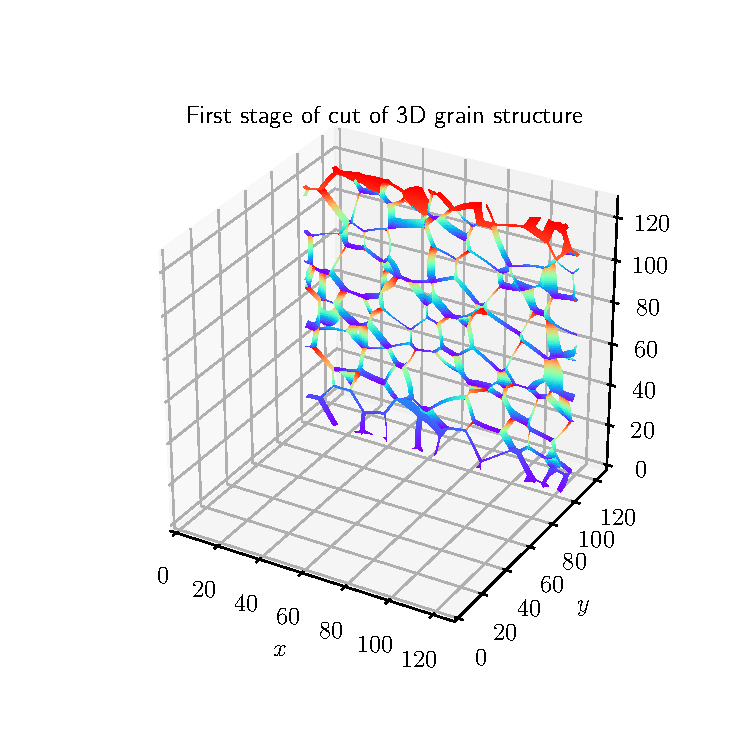
\includegraphics[scale=0.7]{1_cut.pdf}
    \caption{Cut of a cubic grain structure at level $y=100$. An extra plane was added at $y=102$ to clearly show the faces.}
    \label{fig:1_cut}
\end{figure}

The original data comes from a small grid (for example $(128,128,128)$ pixels), therefore the initial cut is expanded by some factor to obtain a bigger image. Knowing the plane we want to obtain, we recover the discrete data that lies in this plane, obtaining a clean two dimensional description as shown in Figure \ref{fig:2_discrete}.

\begin{figure}[h]
    \centering
    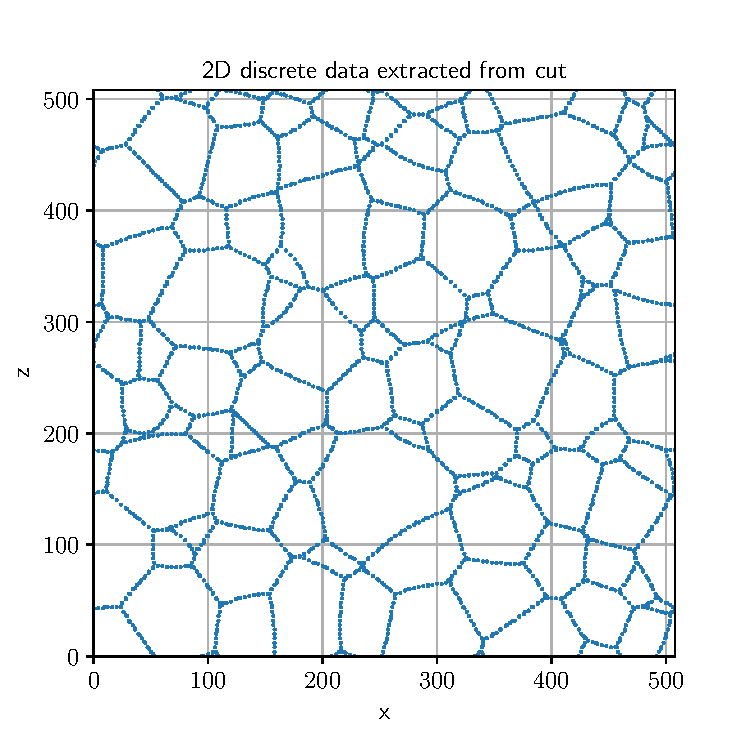
\includegraphics[scale=0.7]{2_discrete.pdf}
    \caption{Discrete representation of a 2D cut.}
    \label{fig:2_discrete}
\end{figure}

Finally, in order to generate a discrete representation with complete boundaries, \ie without discontinuities along boundaries, the obtained data is processed with two image analysis tools: dilation and skeletonize. Dilation operation allows the structure to fullfil the holes in grain boundaries, but this generates very thick boundaries. Skeletonize operation allows to obtain the \emph{skeleton} of the dilated image, obtaining a clean picture of grain boundaries as shown in Figure \ref{fig:3_full_cut}

\begin{figure}[h]
    \centering
    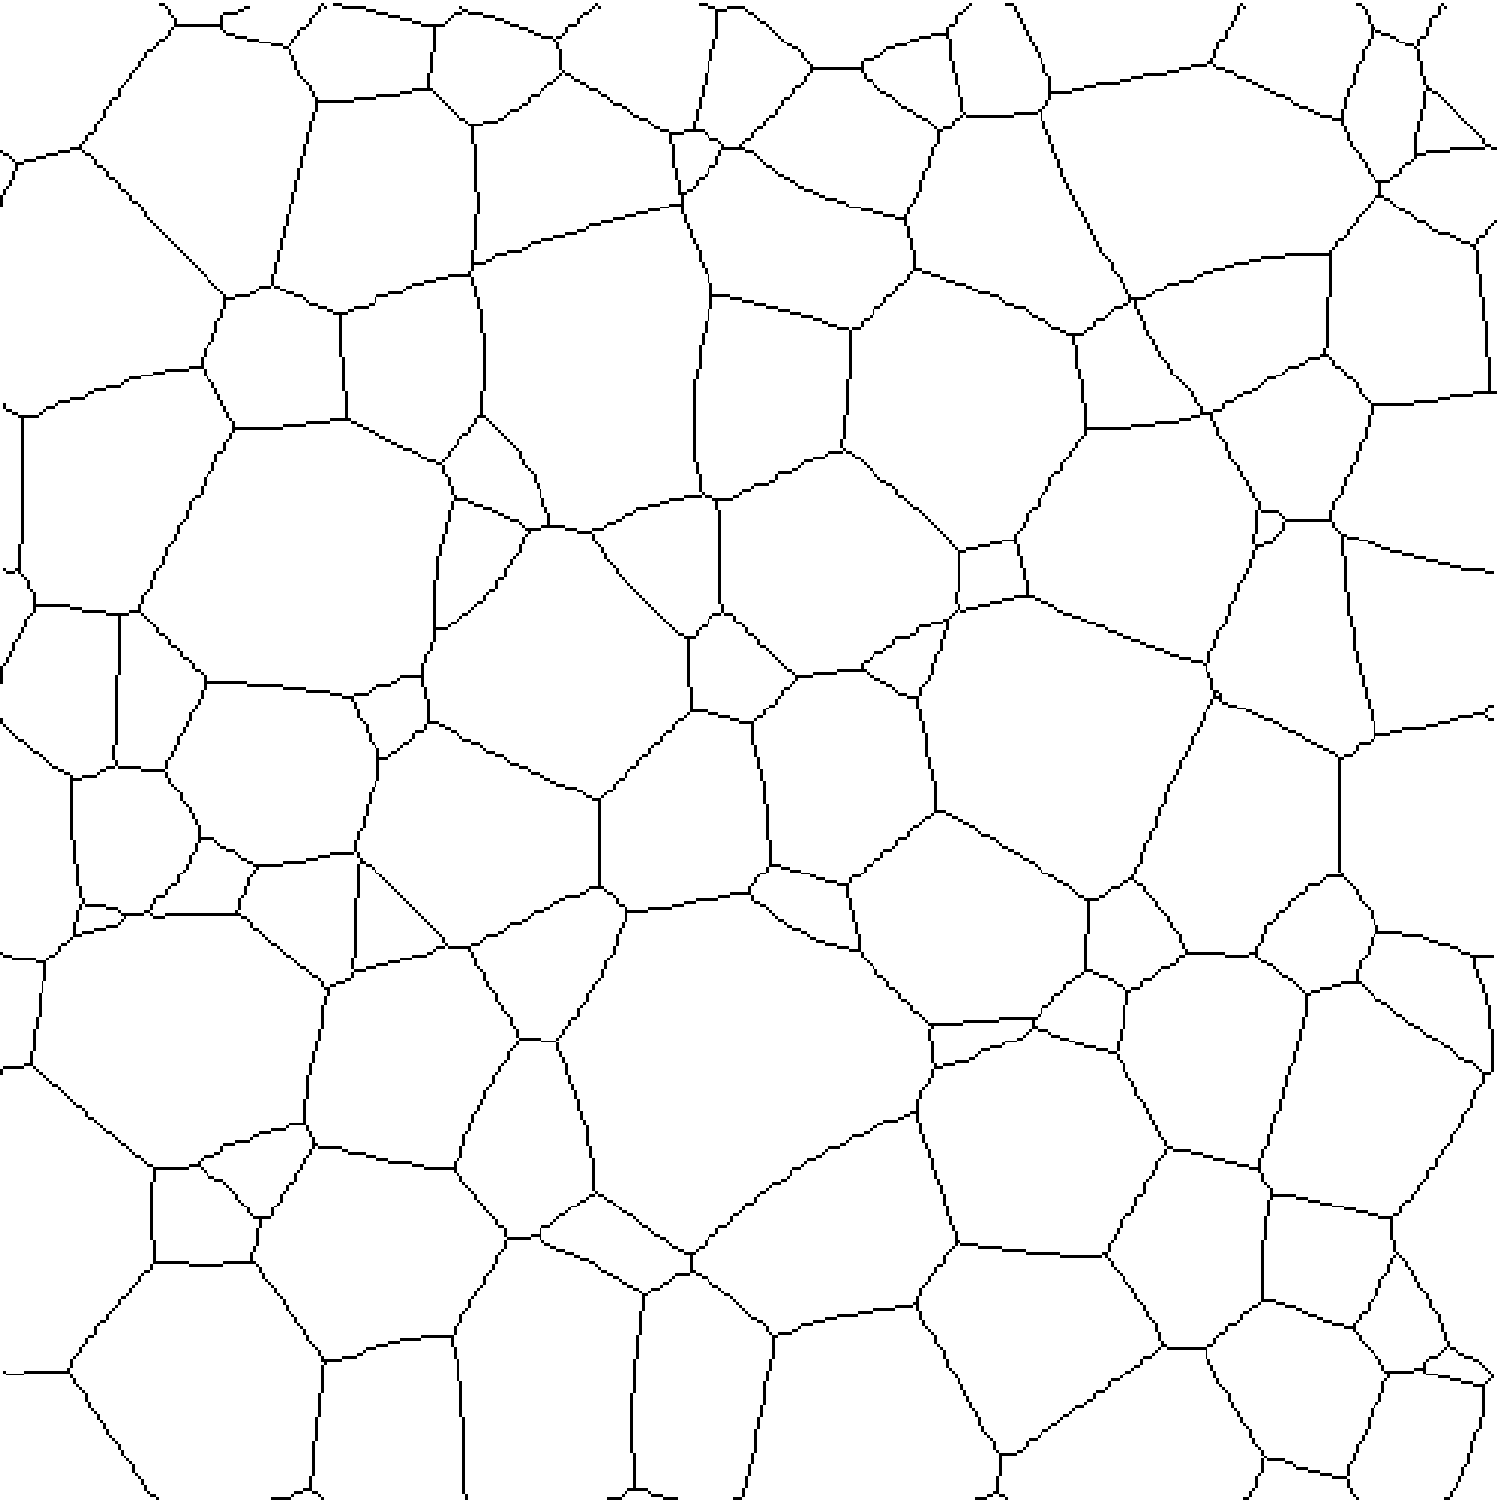
\includegraphics[scale=0.25]{3_full_cut.pdf}
    \caption{Continuous 2D cut.}
    \label{fig:3_full_cut}
\end{figure}

Using the image analysis software ImageJ \cite{schneider2012nih} we can obtain statistics of grain structure. For example ImageJ can obtain grain areas as shown in Figure \ref{fig:4_grains}. The related area distribution is shown in  Figure \ref{fig:5_area_histogram}

\begin{figure}[h]
    \centering
    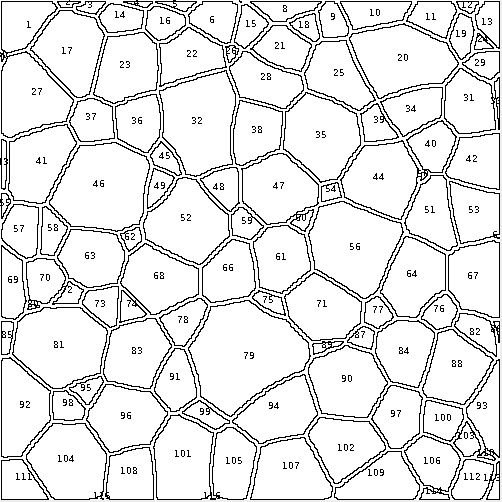
\includegraphics[scale=0.4]{4_grains.png}
    \caption{Grain areas detected by ImageJ software.}
    \label{fig:4_grains}
\end{figure}

\begin{figure}[h]
    \centering
    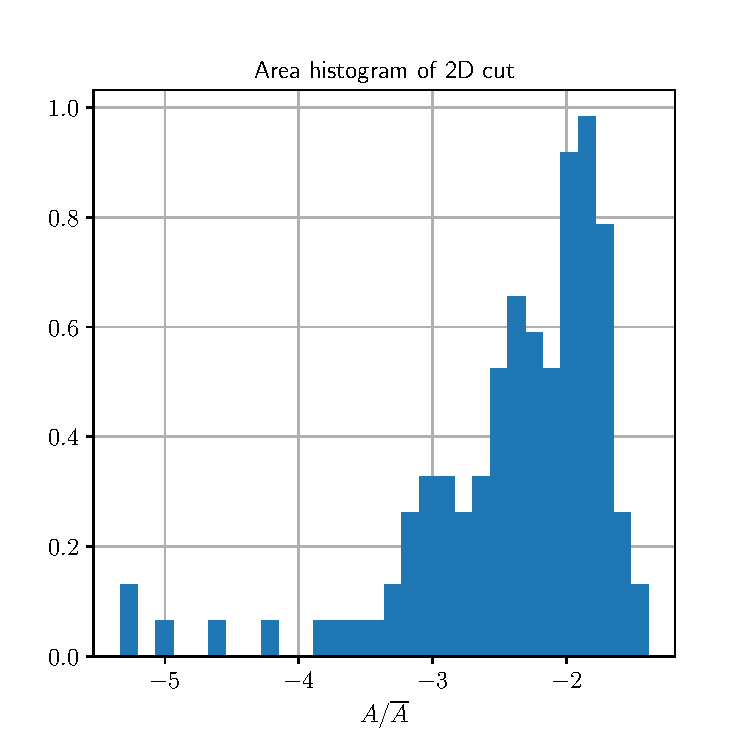
\includegraphics[scale=0.7]{5_area_histogram.pdf}
    \caption{Histogram of relative areas (log scale) for a 2D cut.}
    \label{fig:5_area_histogram}
\end{figure}
